\section{ANÁLISIS DEL GOBIERNO DE TI}
%%%%%%%%%%%%%%%%%%%%%%%%%%%%%%%%%%%%%%%%%%%%%%%%%%%%%%%%%%%%%%%%%%%%%%%%%%%%%%%%%
%	                   Políticas de TI 
%%%%%%%%%%%%%%%%%%%%%%%%%%%%%%%%%%%%%%%%%%%%%%%%%%%%%%%%%%%%%%%%%%%%%%%%%%%%%%%%%

\subsection{Estrategias de las TIs alineadas a las estrategias de la organización}
Las estrategias de TI alineadas a las estrategias de la organización de Alicorp deben enfocarse en potenciar la capacidad de la empresa para cumplir con su misión y alcanzar su visión de liderazgo en los mercados. A continuación, se presentan algunas estrategias clave:

    \subsubsection*{Digitalización y Automatización de Procesos:}
        \begin{itemize}
            \item Objetivo: Mejorar la eficiencia operativa y la calidad de los servicios, alineado con la misión de transformar mercados y generar experiencias extraordinarias.
            \item Estrategia de TI: Implementar soluciones de automatización y digitalización a través de SAP HANA, lo que permite un procesamiento más rápido de datos, optimización de la cadena de suministro y mejor toma de decisiones en tiempo real.
        \end{itemize}
    \subsubsection*{Innovación Tecnológica Continua:}
        \begin{itemize}
            \item Innovar constantemente para generar valor y bienestar en la sociedad.
            \item Estrategia de TI: Integrar tecnologías emergentes como inteligencia artificial, machine learning y análisis avanzado de datos para anticipar tendencias del mercado, personalizar las experiencias del consumidor y optimizar la producción y distribución.
        \end{itemize}

    \subsubsection*{Escalabilidad y Flexibilidad en la Infraestructura:}
        \begin{itemize}
            \item Objetivo: Soportar el crecimiento y expansión en nuevos mercados, contribuyendo a la visión de ser líderes en los mercados en los que competimos.
            \item Estrategia de TI: Adoptar una arquitectura basada en la nube, como Google Cloud Platform, que permita a Alicorp escalar sus operaciones y adaptarse rápidamente a las demandas de los diferentes mercados, asegurando la continuidad y resiliencia del negocio.
        \end{itemize}

    \subsubsection*{Seguridad y Cumplimiento Normativo:}
        \begin{itemize}
            \item Objetivo: Proteger la integridad de los datos y asegurar el cumplimiento con las normativas locales e internacionales, lo que es crucial para operar en múltiples países.
            \item Estrategia de TI: Implementar soluciones de ciberseguridad avanzadas y procesos de gestión de riesgos, junto con auditorías y controles regulares para asegurar que todas las operaciones de TI cumplan con los estándares globales y regionales.
        \end{itemize}

%%%%%%%%%%%%%%%%%%%%%%%%%%%%%%%%%%%%%%%%%%%%%%%%%%%%%%%%%%%%%%%%%%%%%%%%%%%%%%%%%
%	                   Estructura organizacional de la TIC, el CIO y marcos
%%%%%%%%%%%%%%%%%%%%%%%%%%%%%%%%%%%%%%%%%%%%%%%%%%%%%%%%%%%%%%%%%%%%%%%%%%%%%%%%%


\subsection{Estructura organizacional de la TIC, el CIO y marcos}
    \begin{figure}[!ht]
        \centering
        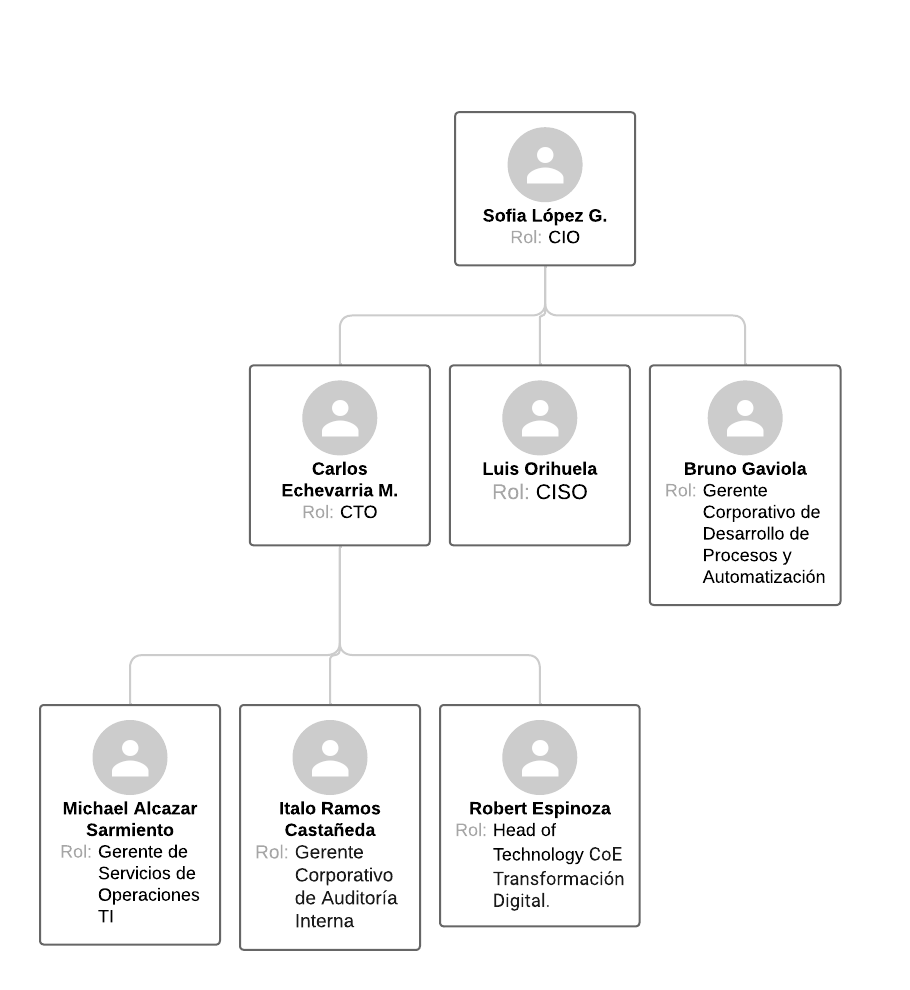
\includegraphics[width=0.8\textwidth]{organigrama_ CIO_TIC.png}
        \caption{Estructura organizacional de la TIC}
    \end{figure}




%%%%%%%%%%%%%%%%%%%%%%%%%%%%%%%%%%%%%%%%%%%%%%%%%%%%%%%%%%%%%%%%%%%%%%%%%%%%%%%%%
%	                   Políticas de TI 
%%%%%%%%%%%%%%%%%%%%%%%%%%%%%%%%%%%%%%%%%%%%%%%%%%%%%%%%%%%%%%%%%%%%%%%%%%%%%%%%%

\subsection{CIO}
    \subsubsection{Perfil de un CIO}
    El perfil de un CIO (Chief Information Officer) en una organización de gran tamaño debe reunir una sólida formación en tecnologías de la información, una visión estratégica clara y habilidades de liderazgo excepcionales. Este ejecutivo debe contar con una experiencia comprobada en la implementación de soluciones tecnológicas innovadoras que optimicen los procesos operativos y faciliten la transformación digital de la empresa. Además, es esencial que tenga la capacidad de liderar equipos multidisciplinarios, manejar proyectos tecnológicos complejos y comunicarse eficazmente con las diferentes partes involucradas. 
    El CIO debe estar preparado para identificar y adoptar nuevas tecnologías de manera proactiva, que impulsen la eficiencia y competitividad de la compañía, garantizando al mismo tiempo la seguridad de la información y el cumplimiento de las normativas vigentes. También es crucial que mantenga una mentalidad estratégica que asegure la alineación de la tecnología con los objetivos corporativos, así como la creación de alianzas estratégicas con proveedores y socios clave. En resumen, el CIO ideal debe ser un líder visionario, con una sólida formación técnica y una clara orientación hacia la innovación y la eficiencia en la implementación de soluciones tecnológicas. 
        \paragraph*{Especificaciones del Perfil }
        \begin{itemize}
            \item Experiencia previa en la implementación de soluciones tecnológicas en la industria de consumo masivo, debe haber liderado proyectos exitosos en la implementación de tecnología para optimizar la cadena de suministro, la producción y la distribución de productos en empresas de gran escala. Es esencial tener un historial comprobado en la mejora de procesos logísticos, automatización de plantas y sistemas de distribución. 
            \item Conocimiento profundo de las tecnologías de la información aplicadas a la producción y logística, debe estar familiarizado con tecnologías como IoT, automatización industrial, inteligencia artificial y análisis de datos, plataformas de gestión de inventario y logística, así como sistemas ERP y CRM utilizados en la industria de consumo masivo. 
            \item Habilidades de liderazgo comprobadas en entornos complejos y de alto rendimiento, debe ser capaz de liderar equipos multidisciplinarios que incluyan profesionales de TI, ingeniería, y operaciones, creando un ambiente colaborativo y orientado a resultados dentro de una industria que opera a gran escala. 
            \item Experiencia en la gestión de la seguridad de la información y protección de datos en un entorno de operaciones complejas, asegurar el cumplimiento de las normativas de seguridad de la información y la protección de datos, en especial en la privacidad del cliente y la integridad de los sistemas de producción y distribución. 
            \item Capacidad para desarrollar e implementar estrategias tecnológicas alineadas con los objetivos de crecimiento de la empresa, debe ser capaz de impulsar la innovación tecnológica que mejore la eficiencia de la producción y la distribución, optimizando procesos operativos y mejorando la agilidad en la respuesta a las demandas del mercado. 
            \item Excelentes habilidades de comunicación, es crucial que pueda colaborar eficazmente con otros líderes empresariales dentro de la organización, como las áreas de operaciones, finanzas y marketing, así como interactuar con socios estratégicos y proveedores clave en el sector de tecnología. 
            \item Experiencia en la gestión de proyectos tecnológicos complejos dentro del sector de alimentos y productos de consumo masivo: El CIO debe asegurar que los proyectos tecnológicos, como la modernización de plantas de producción o la implementación de sistemas logísticos, se entreguen a tiempo y dentro del presupuesto. 
            \item Visión estratégica para identificar oportunidades de crecimiento y optimización tecnológica: Debe poder proponer y liderar iniciativas tecnológicas que maximicen la eficiencia y el crecimiento del negocio, centrando en la sostenibilidad y la innovación en la producción y distribución de productos. 
            \item Entendimiento profundo de los desafíos del sector de consumo masivo: El CIO debe estar familiarizado con las particularidades del mercado, las tendencias de consumo y los desafíos que enfrenta una empresa de la escala de Alicorp, siendo capaz de ofrecer soluciones tecnológicas que potencien su competitividad y liderazgo en el mercado. 
        \end{itemize}
%%%%%%%%%%%%%%%%%%%%%%%%%%%%%%%%%%%%%%%%%%%%%%%%%%%%%%%%%%%%%%%%%%%%%%%%%%%%%%%%%
%	                   Políticas de TI 
%%%%%%%%%%%%%%%%%%%%%%%%%%%%%%%%%%%%%%%%%%%%%%%%%%%%%%%%%%%%%%%%%%%%%%%%%%%%%%%%%

\subsection{Marcos de referencia}

    \subsubsection{COBIT2019}

    Es un marco de gobernanza y gestión de TI que proporciona directrices para el control y la gestión de los procesos de tecnología de la información. Se centra en la creación de valor y en la mitigación de riesgos mediante la implementación de controles efectivos. COBIT ayuda a las organizaciones a garantizar que los procesos de TI estén alineados con los objetivos empresariales, cumplan con los requisitos legales y regulatorios, y proporcionen información precisa para la toma de decisiones. Incluye prácticas para la planificación, evaluación, y monitoreo de TI, así como para la gestión de riesgos, la protección de la información y la eficiencia operativa.Los puntos clave son:
        \begin{itemize}
            \item Gobernanza y Control: Establece un marco para la supervisión y control de los procesos de TI, asegurando que se alineen con los objetivos estratégicos de la organización.
            \item Alineación con Objetivos Empresariales: Garantiza que los procesos de TI respalden los objetivos y necesidades del negocio, facilitando la integración de TI en la estrategia corporativa.
        \end{itemize}

        \begin{figure}[!ht]
            \centering
            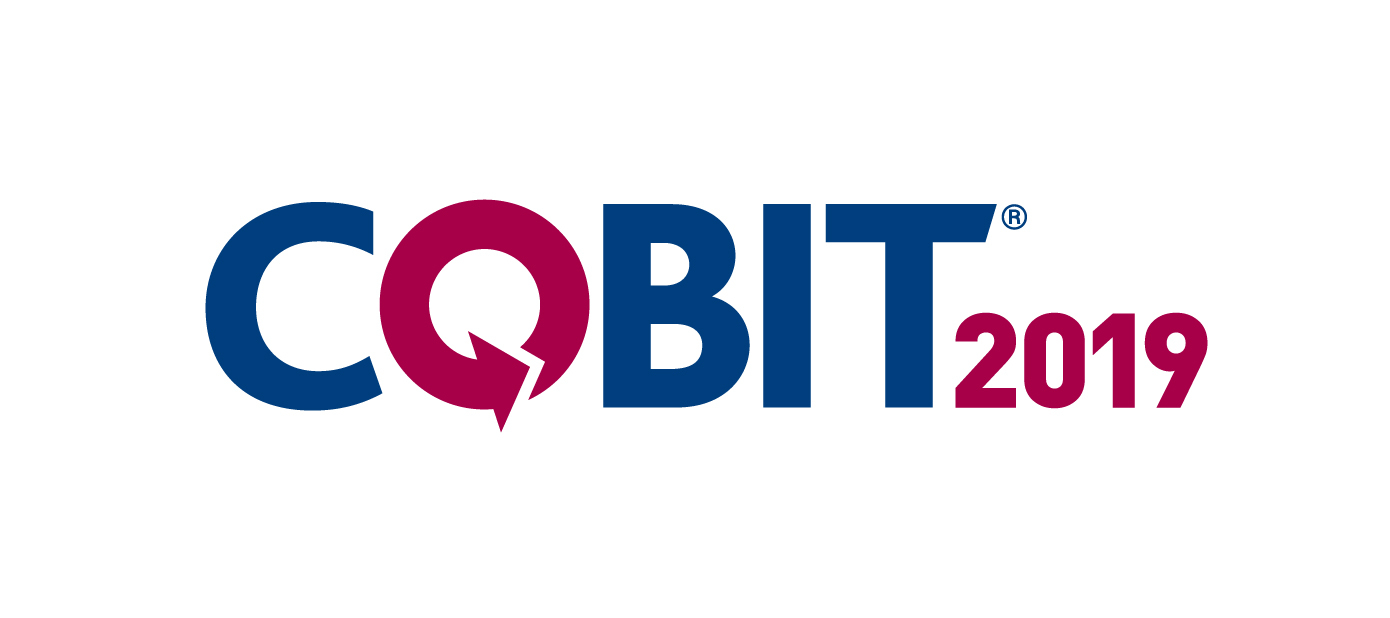
\includegraphics[width=0.8\textwidth]{COBIT2019_logo.jpg}
            \caption{COBIT2019}
        \end{figure}

    \subsubsection{ ITIL v4}

    ITIL es un conjunto de mejores prácticas para la gestión de servicios de TI que se centra en proporcionar un marco para la entrega de servicios de alta calidad. Incluye procesos estandarizados para la gestión de incidentes, problemas, cambios, liberaciones y configuraciones, entre otros. ITIL ayuda a las organizaciones a mejorar la eficiencia operativa, reducir costos, y aumentar la satisfacción del cliente mediante la estandarización de procedimientos y la alineación de los servicios de TI con las necesidades del negocio. Además, ITIL promueve la mejora continua de los servicios a través de un ciclo de retroalimentación y evaluación constante.

    \begin{itemize}
        \item Mejores Prácticas en Gestión de Servicios: Proporciona un conjunto de directrices para gestionar servicios de TI de manera efectiva y eficiente.
        \item Mejora Continua: Promueve la evaluación y optimización continua de los procesos de servicio para mejorar la satisfacción del cliente y reducir costos.
    \end{itemize}

    \begin{figure}[!ht]
        \centering
        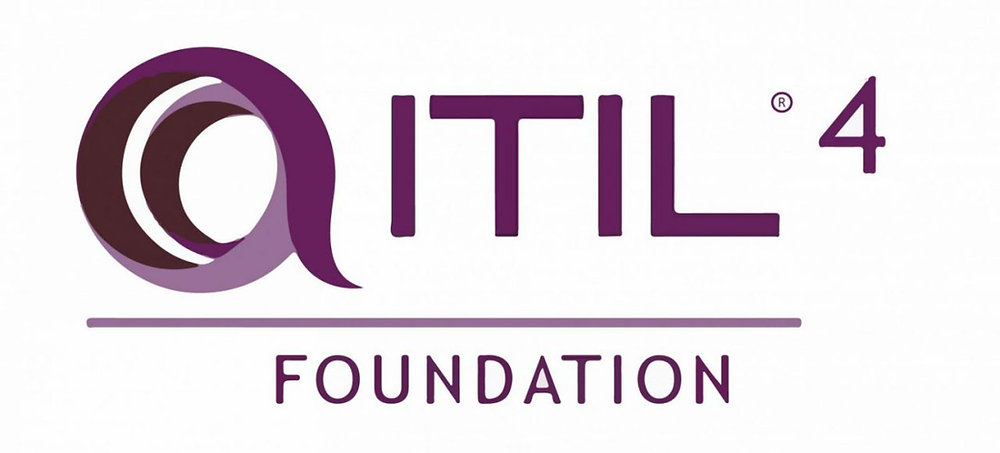
\includegraphics[width=0.8\textwidth]{ITIL_logo.jpg}
        \caption{ITIL}
    \end{figure}

    \subsubsection{TOGAF (The Open Group Architecture Framework)}
    Marco de referencia para el desarrollo y la gestión de la arquitectura empresarial. Proporciona una metodología detallada y un conjunto de herramientas para diseñar, planificar, implementar y gobernar la arquitectura de TI de una organización. TOGAF facilita la alineación de la arquitectura de TI con los objetivos estratégicos del negocio mediante un enfoque estructurado conocido como el ADM (Architecture Development Method). Este marco ayuda a las organizaciones a diseñar una infraestructura de TI que sea flexible, escalable y adaptable a cambios futuros, además de asegurar que todos los componentes tecnológicos funcionen en armonía para apoyar las estrategias empresariales.




%%%%%%%%%%%%%%%%%%%%%%%%%%%%%%%%%%%%%%%%%%%%%%%%%%%%%%%%%%%%%%%%%%%%%%%%%%%%%%%%%
%	                   Políticas de TI 
%%%%%%%%%%%%%%%%%%%%%%%%%%%%%%%%%%%%%%%%%%%%%%%%%%%%%%%%%%%%%%%%%%%%%%%%%%%%%%%%%

\subsection{Estructura organizacional de la TI, sus procesos y funciones}
    \subsubsection{Descripción de las áreas TI}
        \paragraph{Área de TI}
        El área de TI en Alicorp es el pilar tecnológico que impulsa la eficiencia y la innovación en la empresa. Su rol principal es diseñar, implementar y mantener la infraestructura tecnológica necesaria para las operaciones diarias. Esto incluye desde la gestión de redes y servidores hasta el desarrollo de software a medida y el análisis de grandes volúmenes de datos. 
        La TI en Alicorp es mucho más que un simple departamento de soporte. Es un socio estratégico que contribuye al éxito de la empresa de diversas maneras. Automatiza procesos, mejora la toma de decisiones, optimiza la cadena de suministro y fortalece la relación con los clientes. Además, fomenta una cultura de innovación constante, explorando nuevas tecnologías y tendencias del mercado. 
    
        \paragraph{Área de Infraestructura de TI}
        El Área de Infraestructura de TI en Alicorp es la base sobre la cual se construye toda la operación tecnológica de la empresa. Es la división encargada de diseñar, implementar y mantener la red de sistemas, servidores, almacenamiento de datos y demás componentes hardware que permiten el funcionamiento óptimo de las aplicaciones y servicios de la compañía. 
        La infraestructura de TI es como el esqueleto de un cuerpo humano. Mientras que las aplicaciones y software son los órganos que permiten realizar las tareas, la infraestructura es la estructura que los sostiene y conecta. En Alicorp, esta área se encarga de que todos los componentes tecnológicos trabajen en conjunto de manera eficiente y segura. 
    
        \paragraph{Área de Proyectos de TI}
        El Área de Proyectos de TI en Alicorp es el corazón pulsante de la transformación digital de la empresa. Es el equipo encargado de concebir, planificar y ejecutar iniciativas tecnológicas que buscan optimizar procesos, mejorar la eficiencia y generar valor para el negocio. 
        El área de proyectos de TI se puede visualizar como un taller de construcción. Mientras que la infraestructura es el edificio, los proyectos son las reformas y ampliaciones que lo modernizan y adaptan a las nuevas necesidades. Estos proyectos pueden ir desde la implementación de un nuevo sistema de gestión de inventario hasta el desarrollo de una plataforma de comercio electrónico. 
        Para llevar a cabo sus proyectos, el área de proyectos de TI en Alicorp utiliza metodologías ágiles como Scrum o Kanban. Estas metodologías permiten una mayor flexibilidad, adaptabilidad y colaboración entre los equipos, lo que facilita la entrega de valor de manera incremental. 
    
        \paragraph{Área de Mantenimiento}
        El área de mantenimiento de software en Alicorp es el equipo encargado de asegurar que todas las aplicaciones y sistemas informáticos de la empresa funcionen de manera correcta y eficiente. Es como un equipo de médicos especializados en tecnología, que diagnostican, tratan y previenen "enfermedades" en el software. 
        Imaginemos el software como un automóvil. Al igual que un auto necesita revisiones periódicas y reparaciones para mantenerlo en buen estado, las aplicaciones de Alicorp también requieren de un mantenimiento constante. El equipo de mantenimiento de software se encarga de realizar estas revisiones, solucionar problemas y actualizar el software para adaptarlo a las nuevas necesidades del negocio. 
        Las principales funciones del área de mantenimiento de software radican en la corrección de errores, donde se identifica y soluciona los errores o bugs que puedan surgir en las aplicaciones, evitando que afecten el funcionamiento normal del sistema. También están las actualizaciones, es decir, los parches de seguridad y actualizaciones para mejorar el rendimiento y la seguridad del software. Además, se trabaja con una cultura de mejora continua, realizando mejoras en las aplicaciones para aumentar su eficiencia y funcionalidad. 
        Es importante utilizar herramientas y metodologías para llevar estas funciones, por eso existe un sistema de control de versiones que permiten gestionar los cambios en el código fuente de las aplicaciones y entornos de desarrollo integrados que facilitan la programación y depuración de código. Por último, es necesario hablar de las herramientas de automatización, tales como scripts y programas que automatizan tareas repetitivas, como la generación de informes o la ejecución de pruebas. 


%%%%%%%%%%%%%%%%%%%%%%%%%%%%%%%%%%%%%%%%%%%%%%%%%%%%%%%%%%%%%%%%%%%%%%%%%%%%%%%%%
%	                   Políticas de TI 
%%%%%%%%%%%%%%%%%%%%%%%%%%%%%%%%%%%%%%%%%%%%%%%%%%%%%%%%%%%%%%%%%%%%%%%%%%%%%%%%%


\subsection{Políticas TI}
    \begin{figure}[!ht]
        \centering
        \href{https://klintex.com.pe/wp-content/uploads/2021/12/Politica-Privacidad_-Klintex.pdf}{
                
\includegraphics[width=0.25\textwidth]{icon_pdf.png}
                }
    \end{figure}    
%%%%%%%%%%%%%%%%%%%%%%%%%%%%%%%%%%%%%%%%%%%%%%%%%%%%%%%%%%%%%%%%%%%%%%%%%%%%%%%%%
%	                   Objetivos de TI
%%%%%%%%%%%%%%%%%%%%%%%%%%%%%%%%%%%%%%%%%%%%%%%%%%%%%%%%%%%%%%%%%%%%%%%%%%%%%%%%%

\subsection{Objetivos de TI}
    \begin{itemize}
        \item Completar la migración de la empresa de logística en El Salvador de SAP ERP (ECC 6.0) a SAP S/4HANA, asegurando una integración sin fisuras y la eliminación de problemas de transferencia de datos entre sistemas. 
        \item Actualizar las APIs utilizadas en el módulo de gestión de la cadena de suministro (SCM) para mejorar la sincronización de datos en tiempo real y reducir los retrasos en la gestión de pedidos, aumentando la eficiencia operativa. 
        \item Aumentar el ancho de banda de la red en El Salvador y actualizar los routers a equipos más modernos, como los Cisco ISR 4000, para reducir la latencia y mejorar la estabilidad y capacidad de la red durante horas pico. 
        \item Migrar de un sistema de sincronización de datos batch a uno en tiempo real para procesos críticos de la cadena de suministro y logística, garantizando la actualización instantánea de pedidos y el estado de inventarios. 
        \item Implementar un sistema de monitoreo continuo para detectar y resolver proactivamente problemas de sincronización de datos y de red, minimizando el impacto en las operaciones logísticas. 
        \item Desarrollar un equipo de soporte técnico especializado en El Salvador, capacitado para resolver de manera rápida y eficiente cualquier problema relacionado con TI y la infraestructura de red, asegurando la continuidad del servicio. 
        \item Optimizar la red VPN privada utilizada en El Salvador para reducir la latencia a menos de 150 ms durante horas pico y garantizar un ancho de banda suficiente para soportar las operaciones críticas de logística. 
        \item Desarrollar e implementar un plan de contingencia robusto que permita a Alicorp mantener la continuidad operativa en El Salvador frente a posibles interrupciones en la red o fallas en el sistema, minimizando el impacto en la cadena de suministro y la satisfacción del cliente.
    \end{itemize}
%%%%%%%%%%%%%%%%%%%%%%%%%%%%%%%%%%%%%%%%%%%%%%%%%%%%%%%%%%%%%%%%%%%%%%%%%%%%%%%%%
%	                   Organización del área de TI
%%%%%%%%%%%%%%%%%%%%%%%%%%%%%%%%%%%%%%%%%%%%%%%%%%%%%%%%%%%%%%%%%%%%%%%%%%%%%%%%%

\subsection{Organización del área de TI}
\begin{figure}[!ht]
    \centering
    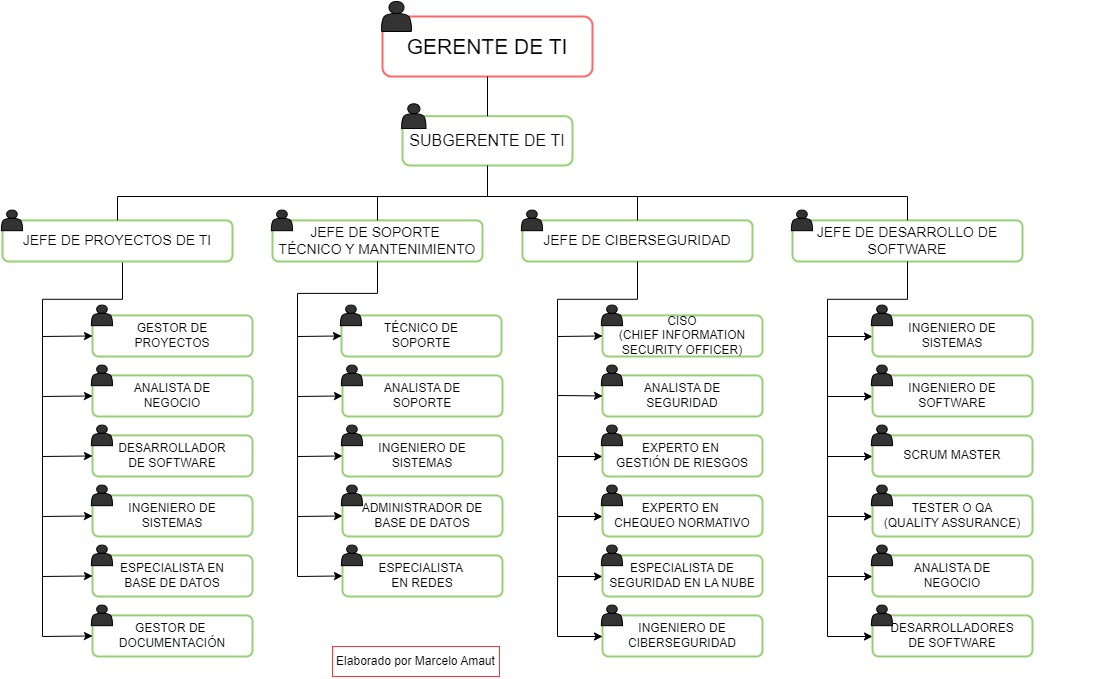
\includegraphics[width=0.8\textwidth]{estructura_organizacional_alicorp.jpeg}
    \caption{Organigrama  de la organización del área de TI}
\end{figure}
    \subsubsection{Funciones}
    \begin{itemize}
        \item Desarrollo y Mantenimiento de Sistemas: Asegurar el funcionamiento continuo y eficiente de las aplicaciones empresariales, incluyendo SAP y otras plataformas críticas.
        \item Gestión de Infraestructura: Supervisar la infraestructura tecnológica, incluidas redes, servidores y almacenamiento, para garantizar una alta disponibilidad y rendimiento.
        \item Seguridad de TI: Implementar y gestionar políticas de seguridad para proteger los datos y sistemas de la empresa contra amenazas y vulnerabilidades.
        \item Soporte Técnico: Proporcionar soporte a los usuarios internos para resolver problemas técnicos y garantizar el uso óptimo de las herramientas tecnológicas.
    \end{itemize}
    \subsubsection{Responsabilidades}
    \begin{itemize}
        \item Chief Information Officer (CIO): Define la estrategia tecnológica de la empresa, asegura la alineación de TI con los objetivos empresariales y supervisa la ejecución de proyectos clave.
        \item Gerente de Infraestructura TI: Administra la infraestructura tecnológica, incluyendo redes, servidores y almacenamiento, para mantener la operatividad y escalabilidad de los sistemas.
        \item Gerente de Servicios de Operaciones TI: Supervisa la operación diaria de los sistemas de TI, incluyendo el soporte técnico y la gestión de incidentes, para asegurar un servicio continuo y eficiente.
        \item Arquitecto de TI: Diseña y mantiene la arquitectura tecnológica de la empresa, asegurando que las soluciones tecnológicas se alineen con la estrategia de negocios y los estándares de la industria.
        \item Especialista en Seguridad de TI: Desarrolla y aplica políticas de seguridad, gestiona riesgos y asegura el cumplimiento de normativas de seguridad para proteger los activos digitales de la empresa.
    \end{itemize}